By scaling model capacity and training on massive, diverse text corpora, large language models (LLMs) have demonstrated strong capabilities in language understanding, knowledge generalization, and conversational dialogue~\cite{hu2024survey}. These capabilities have motivated growing interest in deploying LLMs as planning agents that can perceive an environment, reason about possible actions, and make decisions in interactive tasks compared with the traditional deep reinforcement learning (DRL) based method~\cite{park2025optimizing}. Among these tasks, navigation provides a useful scenario because it requires an agent to interpret the ego and neighbors states, avoid hazards, maintain short-term memory, and plan towards a goal with a partially observed environment.

Recent studies suggest that LLM-based agents can be effective in sequential decision-making settings, but their performance depends heavily on how reasoning is structured\cite{nourzad2026mira,omelchenko2025reflective}. A purely reactive agent may respond quickly and cheaply, yet struggle in environments that require longer-horizon planning. In contrast, prompting strategies such as Chain of Thought, ReAct, Tree of Thought, and Buffer of Thought may improve decision quality by encouraging explicit reasoning, action evaluation, or memory use. However, these methods also introduce tradeoffs in token cost, inference complexity, and exploration efficiency. As a result, it remains unclear which reasoning strategy is most effective for navigation tasks under different levels of difficulty.

To address this issue, a controlled and comparative study is conducted to identify the effectiveness of different LLM agents, as shown in \figureautorefname~ \ref{fig:framework}. We deploy 5 kinds of LLM agents in the MiniGrid environment with the aspect of memory and reasoning methods. The effectiveness of the 5 methods is discussed in terms of the performance metrics of average success rate, exploration steps, and tokens used.  
The contributions of this study are as follows:

\begin{itemize}
\item \textbf{LLM implementation on navigation.} We design effective prompts and different reasoning methods for the LLM agents to achieve robust decision-making for navigation in the MiniGrid environments.
\item \textbf{Comparative study on LLM agents.} We evaluate the 5 LLM agents in three environments with increased difficulty levels, then compare their success rate and tokens used for model selection guidance.
\end{itemize}
\begin{figure}[htbp]
    \centering
    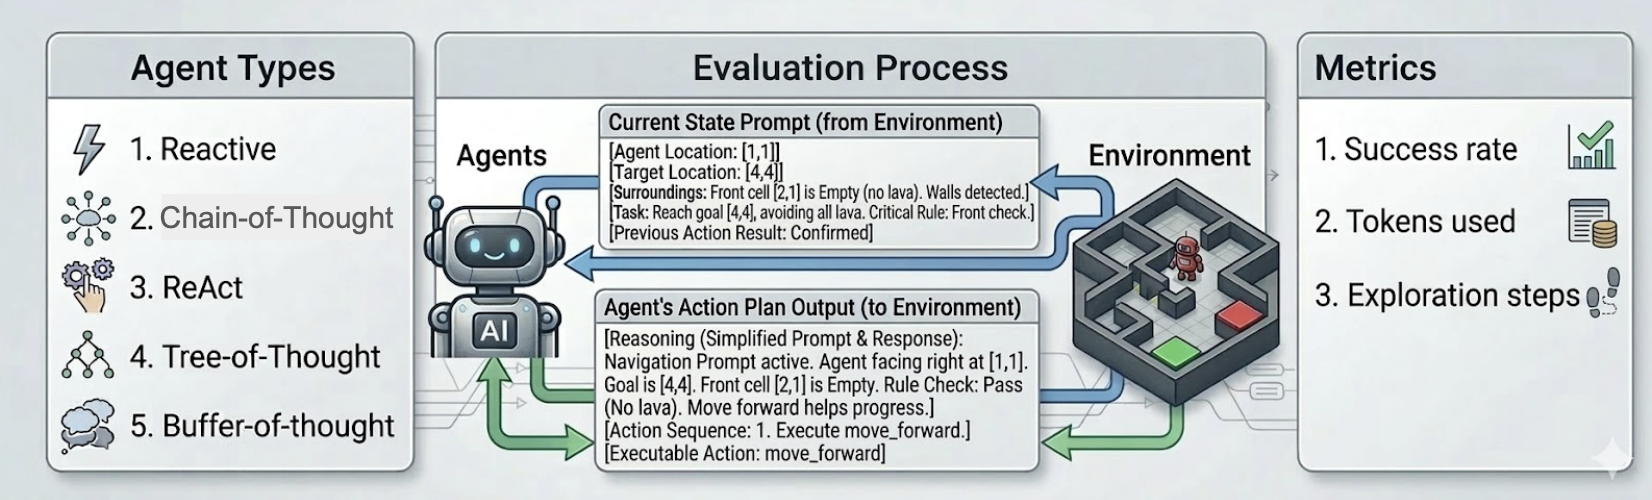
\includegraphics[width=0.9\linewidth]{Figures/Framework.png}
    \caption{The overall framework for the comparative study}
    \label{fig:framework}
\end{figure}